\documentclass{llncs}
\usepackage{llncsdoc}
\usepackage{hyperref}
\usepackage{graphicx}
\usepackage{array}
\usepackage{float}
\usepackage{fancyvrb}
\usepackage{amsmath}
\usepackage{multicol}
\usepackage{mathtools}
\DefineVerbatimEnvironment{code}{Verbatim}{fontsize=\small}
\DefineVerbatimEnvironment{example}{Verbatim}{fontsize=\small}

%
\begin{document}
\title{Dual Degree Project - Interim Report}
\author{Bharath Reddy}
\institute{CS09B030, CSE, IIT Madras}
\maketitle
%
\section{Introduction}
"Which digital camera should I buy? Which movie should I rent? Which book should I buy for my next vacation?" These are some situations where people have to make decisions about how they are going to spend money, or in a broader level, about their future.
Traditionally, people have used a variety of strategies to solve such decision making problems: conversations with friends, obtaining information from a trusted third party, hiring an expert team or simply follow the crowd. It would be great to have an affordable personal advisor who helps us make good decisions efficiently.
The construction of systems that supports a user in his/her (online) decision-making is the main goal of the field of recommender systems. In particular, the goal of recommender systems is to provide easily accessible, high-quality recommendations for a large user community. \\
      Recommender Systems are broadly classified into three categories:
\begin{itemize}
\renewcommand{\labelitemi}{$\bullet$}
\item \textbf{Collaborative recommender systems}: The main idea in these systems is that if users share the same interests in the past - if they viewed or bought the same books - they will also have similar tastes in the future. Items which are not yet seen by the current user, but which are liked by users similar to him are recommended. This technique is also called as \textit{Collaborative Filtering}. Pure CF based approaches do not exploit or require any knowledge about the items themselves.

\item \textbf{Content based recommender systems}: If I know that "Harry Potter" is a fantasy novel and Alice has always like fantasy novels, I can recommend the new "Harry Potter" book right away. 
In content based recommenders, item descriptions along with a user profile that describes the tastes of the user is used to recommend items here

\item \textbf{Knowledge based recommender systems}: Typically, we do not buy a house, a car, 
or a computer very frequently. In such a scenario, a pure CF system will not perform well because of the low number of available ratings
In more complex product domains such as cars, customers often want to define their requirements explicitly - for example, "the maximum price of the car is $x$ and the color should be \textit{black}". In knowledge based systems, recommendations are made taking into account the explicit user preferences and the rich knowledge base available.
\end{itemize}
Recommendation process of knowledge-based recommender applications is highly interactive, a foundational property that is a reason for their characterization as \textit{\textbf{conversational systems}}. The recommender system that we consider in this project is a conversational system.\\
Conversational systems assume that a user's initial query is merely a starting point for search, perhaps even an unreliable starting point. The job of the recommender system is to help the user refine his initial preference query as the interactions proceed.

\textit{\textbf{Critiquing}} is one of the most popular forms of feedback in conversational recommender systems. In each interaction cycle, the user is presented with a list of products.
User selects a product and expresses directional preferences over some particular item feature values. For example, one might indicate that he/she is looking for a less expensive restaurant or a more formal setting. These are two individual critiques, first critique being on the \textit{price} attribute and the second critique on the \textit{setting} attribute. The recommender updates it's user model according to this feedback ;provides another set of products and proceeds to the next recommendation cycle. This continues till the user finally chooses a product.

\textit{\textbf{Unit critiques}} allow users to express their preference over one attribute in each interaction cycle. \textit{\textbf{Compound critiques}} enable users to input their preferences on several attributes at a time. This can potentially shorten the number of interaction cycles in finding a target product.



\section{Background}
      A critical issue for recommender systems relying on compound critiques is to dynamically generate a list of high quality compound critiques in each interaction cycle to save the users' interaction effort. In earlier research, \textbf{Apriori algorithm}, \textbf{Multi Attribute Utility Theory (MAUT)} based methods were used to generate compound critiques on the fly as the interactions proceed.

\textbf{Incremental Critiquing}, proposed by Reilly et.al \cite{reilly} discovers feature patterns that are common to remaining products on every recommendation cycle.
The first step involves \textit{generating critique patterns} for each of the remaining product options in relation to the currently presented example. Figure \ref{fig:critiquePatterns}  shows critique pattern generated for a product $p$ w.r.t. the current reference product.

The next step involves \textit{mining compound critiques} by using the \textit{Apriori algorithm} to identify groups of recurring unit critiques. Apriori returns lists of compound critiques of the form \{[ProcessorSpeed $>$], [Price $>$]\} along with their support values (i.e., the \% of critique patterns for which the compound critique holds)
Compound critiques with low support values eliminate many more products from consideration if chosen. The top $k$ products with lowest support values are displayed to the user.

\begin{figure}
    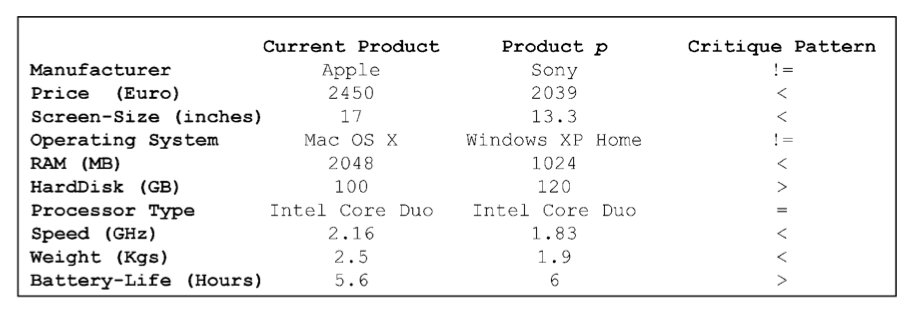
\includegraphics[width=1.0\textwidth]{critiquePatterns.png}
  \caption{Critique Pattern for the product p. Reference: \cite{reilly2007evaluating}}
  \centering
\label{fig:critiquePatterns}
\end{figure}

\textbf{MAUT based critiquing}, proposed by Zhang and Pu \cite{zhang}
uses a simplified weighted additive formula to calculate the utility of a product $O = \langle x_1,\hdots,x_n\rangle$ as follows:
\begin{align*}
U(\langle x_1,\hdots,x_n \rangle) = \sum_{i=1}^n w_iV_i(x_i)
\end{align*}
The system constructs a preference model which contains the weights and the preferred values for the product attributes to represent the user's preferences. At the beginning of the interaction process, the initial weights are equally set to $1/n$ and the initial preferences are stated by the user.

In each iteration,
The MAUT approach first determines the top K (in practice the authors set K = 5) products with maximal utilities, and then each of the top K products are converted into compound critique strings (Eg: Faster CPU, larger hard-disk and longer battery).
When the user selects a compound critique, the corresponding product is assigned as the new reference product, and the user's preference model is updated based on this critique selection.The weight of each attribute is adaptively adjusted (either multiplied or divided by a factor $\beta$ (=2)) according to the difference between the old preference value and the new preference value(attribute value of new reference product). 
Products that were displayed in a this iteration are removed from the case base. 
This continues till the user selects a product.

Reilly et. al \cite{reilly2007evaluating} performed an elobarate user-study to compare the above two approaches. It was observed that both the systems performed equally well w.r.t. most objective (number of interaction cycles, recommendation quality/accuracy) and subjective criteria(such as user's perceived satisfaction) 
%Why is it interesting
%What shortcomings of the Apriori Critiquing does it try to address
%In \cite{zhang}, offline experiments showed that MAUT based critiquing outperformed Apriori based compound critiquing.
% the proposed Critique MAUT approach can reduce the interaction cycles over 20\% compared to the Critique Apriori approach
%In (cite the follow up paper), live user studies were performed and it was shown that MAUT and Apriori critiquing perform similarly in most situations (in terms of number of hops per product)
%Shortcomings

\section{Problem Definition}
\label{sec:problemStmt}
Following are few questions that we aim to explore, experiment and come up with solutions:\\
\begin{enumerate}
\renewcommand{\labelitemi}{$\bullet$}
\item In the user evaluation performed by Reilly et. al. \cite{reilly2004explaining} on the Apriori based critiquing system, many users have given feedback that the critiques weren't diverse enough. 
There has been no work addressing the diversity in critiques to the best of our knowledge.
How can the above techniques be improved so that the critiques can be more diverse?
\item How can the relationship between displayed products be used to quickly arrive at the target product? For example, if item no. 2 was selected in a particular iteration, can we make use of the fact that it was preferred over the items 1,3,4 and 5 to make the procedure faster?
\item Can there be improved results if aggregate attributes (quality, economy etc) are used in computation of utility instead of the basic attributes. Aggregate attributes can be modeled as linear combination of the basic attributes and correlate closely with user's way of thinking - how good product I want (quality) and how much I am willing to pay for that (economy). How can the scoring rules for each attribute be mined from the rich knowledge base or from user interaction logs?
\item Weight Update model in \cite{zhang} looks too simplistic as of now. Can we come up with a new weight update scheme that enables us to quickly arrive at the target
\item In MAUT based recommendation \cite{zhang}, can proposing two items(instead of one) lead to fewer interaction cycles? How should the critique strings in each iteration be changed accordingly?
\item Instead of using the utility scores, can we have linear combination of utility and similarity scores to rank a product?
\end{enumerate}


\section{Impact of Solving the Problem}
Critiquing has been shown to be a very effective way to help na\"{i}ve users with limited domain knowledge nagivate complex item spaces. 
Discovering a technique that reduces the number of interaction cycles to reach the target product saves user's time, improves user experience and decreases cognitive load on the user. 


\section{Work Done Till Date}
\label{sec:workDoneTillDate}
\begin{itemize}
\renewcommand{\labelitemi}{$\bullet$}
\item Read the book "An Introduction to Recommender Systems" by Jannach et.al. \cite{jannach}. The book covers most of the introductory topics on recommender systems
\item Read the chapter "Evaluating Recommender Systems" in "Recommender Systems Handbook" by Shani et.al. ~\cite{shani}. Studied several properties and evaluation procedures for recommender systems
\item Implemented a knowledge based recommender system (in Python), which supports critiquing and preference-based search (Section ~\ref{sec:methodology})
\item Leave-one-out method, a popular offline evaluation mechanism for knowledge based systems has been implemented (Section ~\ref{sec:evaluationProcedure})
\item Conducted experiments by modifying the similarity function and altering weight parameters for different attributes. Utility measures were also included to rank a product
\item Currently reading the paper "On the Evolution of Critiquing Recommenders" by Reilly et.al., which provides an in-depth analysis of how critiquing systems have evolved over the years and the current state-of-the-art critiquing recommender systems

\end{itemize}


\section{Timeline for Future Work}
\begin{itemize}
\renewcommand{\labelitemi}{$\bullet$}
\item November through January: Work on the problems 2,4,5 and 6 in Section ~\ref{sec:problemStmt}.
Test the new system using offline evaluations and compare it with other existing compound critiquing mechansims

\item February through March: Work on problems 1 and 3 in Section ~\ref{sec:problemStmt}. Perform offline tests.

\item April: Create a web interface in collaboration with others to perform user evaluations on the model.

\item May: Write the final report.
\end{itemize}

\section{Experiments}

The following subsections describe the methodology, datasets and evaluation procedure used for the basic recommender system that has been implemented
\subsection{Description of the System}
\label{sec:methodology}
\begin{itemize}
\renewcommand{\labelitemi}{$\bullet$}
\item In the first interaction cycle, user provides his preferences on a single attribute or multiple attributes.
\item Preferences can be specified to be \textit{less-than}, \textit{greater-than} or \textit{around} a particular attribute value (Eg: Camera price should be \textit{less than} \$500, resolution should be \textit{greater than} 8.0MP, zoom should be preferably \textit{around} 4)
\item Similarity between two products is calculated as the sum of weighted similarity between attributes
\begin{equation}
sim(c1, c2) = \sum_{i} w_i*sim(c1({a_i}), c2({a_i})) 
\end{equation}
\begin{equation}
sim(q, c) = \sum_{i \in q} w_i*sim(q({a_i}), c({a_i}))
\end{equation}
In the above equation c1, c2, c denote a case; q denotes a query; $a_i$ denotes the $i^{th}$ attribute of a case

\item Similarity between attribute values for numeric attributes is taken as the inverse of the normalized distance between the two attributes
\begin{equation}
dist(c1({a_i}), c2({a_i})) = \lvert(c1({a_i}) - c2({a_i})) \rvert/range({a_i})
\end{equation}
\begin{equation}
sim(c1({a_i}), c2({a_i})) = 1/(1+dist(c1({a_i}), c2({a_i})))
\end{equation}

\item Similarity between non-numeric attributes is hard-coded. Similarity values derived from real user interaction logs will definitely be more accuracte, but they are unavailable at the moment
\end{itemize}
Along with similarity, we attempt to calculate the utility scores for each product, based on aggregate attributes (like quality and economy for camera domain) . Final score for a product is the weighted sum of utility and similarity scores. The procedure for calculating utility scores is described below:
\begin{itemize}
\renewcommand{\labelitemi}{$\bullet$}
\item Quality and economy (the aggregate attributes for the camera domain) scores for each attribute are computed for a product. Eg: Let product p1 = \{'Price':300, 'Resolution':10, 'OpticalZoom':6, 'DigitalZoom': 10, 'Weight': 400\}. 
From Table ~ \ref{tab:scoringTable}, 
quality score for the p1 = 10+10+6+10+5 = 41, economy score = 5+10+9+10+10 = 44.
\item Customer-specific item utility is calculated on the basis of the formula below:
\begin{equation}
utility(p) = \sum_{j=1}^{\#(dimensions)} interest(j) * contribution(p, j)
\end{equation}
\textit{interest(j)} denotes a user's interest in dimension $j$ , and $contribution(p, j)$ denotes the contribution of item $p$ to the interest dimension $j$
\item If the user specificies the following requirements: REQ = \{r1: Price $\le$ 200; r2: Resolution = 8; Weight $\le$250\}; $interest(j)$ is calculated using the scoring rules in the given table\ref{tab:scoringTable}- Quality = 19, Economy = 25. Normalize $interest(j)$ for quality = 0.43; for economy = 0.57 

\item Final score for the product is computed as a weighted summation of similarity and utility. Items are ranked based on the final scores
\begin{equation}
\label{eq:alpha}
score(p, q) = \alpha*sim(p,q) + (1-\alpha)*utility(p)
\end{equation}
Here p is a product, q can be another product or a query

\end{itemize}

\begin{table}
\caption{Scores for each attribute of a camera wrt the dimensions of quality and economy. Reference: \cite{jannach}, p. 98}
\centering
\setlength{\tabcolsep}{12pt}
\renewcommand{\arraystretch}{1.5}
\label{tab:scoringTable}

    \begin{tabular}{llll}
    \hline
    \hline
    ~            & Value  & Quality & Economy \\
    \hline
    Price        & $\leq$ 250        & 5          & 10      \\
    ~            & $>$ 250         & 10         & 5       \\
    \hline
    Resolution   & $\leq$ 8          & 4          & 10      \\
    ~            & $>$ 8           & 10         & 6       \\
    \hline
    Optical Zoom & $\leq$ 9          & 6          & 9       \\
    ~            & $>$ 9          & 10         & 6       \\
    \hline
    Digital Zoom & $\leq$ 9          & 6          & 10      \\
    ~            & $>$ 9          & 10         & 6       \\
    \hline
    Weight       & $\leq$ 300        & 10         & 5       \\
    ~            & $>$ 300        & 5          & 10      \\
    \hline
    \hline
    \end{tabular}
\end{table}

\subsection{Datasets and Evaluation procedure used}
\label{sec:evaluationProcedure}
\textbf{Dataset used:}
Camera Data Set - \href{http://josquin.cs.depaul.edu/~rburke/research/downloads/camera.zip}{(with 209 Cameras)} \\
Each camera in the data set has 10 attributes:
\renewcommand{\labelitemi}{$\bullet$}
\begin{multicols}{2}
\begin{itemize}
\item Manufacturer
\item Model
\item Price(\$)
\item Format
\item Resolution (M Pixels)
\item Optical Zoom (X)
\item Digital Zoom (X)
\item Weight (grams)
\item Storage Type
\item Storage Included (MB)
\end{itemize}
\end{multicols}
\textbf{Evaluation Procedure}:
The recommender system has been evaluated based on \textit{leave-one-out}, a well-known offline evaluation mechanism for knowledge based systems
The number of preferences($N$) in the query are fixed at a constant (Eg: 1,3,5) at the beginning of evaluation.
A product($C$) is selected from the dataset at random, removed from the dataset and is used for formulating a query.
The product $T$, that has the highest scores(according to Equation~\ref{eq:alpha}), is fixed as the target product for the recommender system.
\textit{Quality} and \textit{Economy} preferences are also fixed according to the test product $T$ and the scoring table~\ref{tab:scoringTable}
$N$ attributes are selected from $C$ and are given as initial user preferences to the recommender system.
Recommender returns 4 top products (scored according to Equation~\ref{eq:alpha}) based on the given preferences.
The recommendation process stops when $T$ appears in the list of recommendations.
If $T$ is not present in the list of recommendations, the simulated user selects the product $P$ that has the highest score (Equation ~\ref{eq:alpha}), and the iterations continue.

Screenshots of the console application for recommendation and evaluation procedures are shown in Appendix ~ \ref{sec:appendix}\\
\textbf{Results}:
Offline evaluations have been conducted for different values of the paramter $\alpha$ in Equation ~\ref{eq:alpha}.
For each value of $\alpha$, leave-one-out method has been performed for 100 times and the average number of hops have been calculated.
Number of attributes in the query in all the experiments = 2. Average number of hops is found to be the least for $\alpha$ = 0.8.
Results are tabulated in Table ~\ref{tab:results}.

\begin{table}
\centering
    \caption{Average Number of Hops vs different values of $\alpha$ in Equation ~\ref{eq:alpha}}
\label{tab:results}
    \begin{tabular}{ >{\centering\arraybackslash} m{4cm} >{\centering\arraybackslash} m{4cm} }
    \hline
    \hline
    $\alpha$ & Average Hops (100 tests) \\
    \hline
    0.1    & 8.3                      \\
    0.2    & 7.7                      \\
    0.3    & 7.86                      \\
    0.4    & 8.4                      \\
    0.5    & 7.96                      \\
    0.6    & 8.3                      \\
    0.7    & 8.17                      \\
    0.8    & 6.4                      \\
    0.9    & 8.24                      \\
    1.0    & 6.9                      \\
    \hline
    \hline
    \end{tabular}

\end{table}

\section{Literature Survey}
\label{sec:litSurvey}
\begin{itemize}
\renewcommand{\labelitemi}{$\bullet$}


\item Linden et.al. \cite{ataSystem} use a constraint solver to obtain a set of optimal solutions in each iteration and show five of them to the user (three optimal ones and two extreme solutions)

\item Reilly et.al \cite{reilly2004explaining} conducted user evaluations on their preliminary compound critiquing algorithm that used the Apriori algorithm. 
Some users gave feedback that the recommender just seemed to \textit{"forget"} their preferences in the next iteration. This lead them to propose the "Incremental Critiquing" \cite{reilly} algorithm, which tries to satisfy as many past user preferences as possible along with preferences currently given through critiquing

\item Reilly et.al \cite{reilly2007evaluating} perform a user-study to compare the performances of Apriori based critiquing algorithm and MAUT based recommendation algorithm. Both the algorithms were found to perform equally well w.r.t most objective (number of interaction cycles, recommendation quality/accuracy) and subjective criteria(such as user's perceived satisfaction) 

\item Books mentioned in Section ~\ref{sec:workDoneTillDate}
\end{itemize}


%First incremental critiquing
%Some more simple critiquing papers?
%What about "Preference based search using Example Critiquing" Viappiani
%May be look up for some more papers which cite the "MAUT BASED COMPOUND CRITIQUING" paper

\section{Discussion}
\label{sec:discussion}
\subsection{Evaluation of Recommender Systems}
There are three different types of experiments for evaluating recommender systems; offline, user studies and online experiments.\\
\textbf{Offline Experiments:}
An offline experiment is performed by using a pre-collected data set of items\\
%The goal of the offline experiments is to filter out inappropriate ap- proaches, leaving a relatively small set of candidate algorithms to be tested by the more costly user studies or online experiments. A typical example of this process is when the parameters of the algorithms are tuned in an offline experiment, and then the algorithm with the best tuned parameters continues to the next phase.
\textbf{User Studies:}
A user study is conducted by recruiting a set of test subjects, and asking them to perform several tasks requiring an interaction with the recommendation system \\
%To test all candidates we can either compare the candidates \textit{\textbf{between subjects}}, where each subject is assigned to a candidate method and experiments with it, or \textit{\textbf{within subjects}}, where each subject tests a set of candidates on different tasks
%Typically, \textit{within subjects} experiments are more informative, as the superiority of one method cannot be explained by a biased split of users between candidate methods
%\textit{Between subjects} experiments, also known as A-B testing (All Between), provide a setting that is closer to the real system, as each user experiments with a single system 
\textbf{Online Experiments:}
Online experiments are large scale experiments on a deployed system. Such experiments evaluate the performance of the recommenders on real users who are oblivious to the conducted experiment.
%\subsubsection{Recommender System Properties:}
%Following are some of the properties considered when deciding which recommendation approach to select.As different applications have different needs, the designer of the system must decide on the important proper- ties to measure for the concrete application at hand.
%\renewcommand{\labelitemi}{$\bullet$}
%\begin{multicols}{2}
%\begin{itemize}
%\item Prediction Accuracy
%\item Coverage
%\item Confidence
%\item Trust
%\item Novelty
%\item Serendepity
%\item Diversity
%\item Utility
%\item Adaptivity
%\item Scalability
%\end{itemize}
%\end{multicols}


\subsection{Online Consumer Decision Making}
\label{sec:onlineConsumerDecisionMaking}
Traditional models of human decision making are based on the assumption that consumers make optimal decisions on the basis of rational thinking. 
These models assume that the perceived utility of one product in a list is unaffected by the presence of other items in the list. 
But recent research done in the area of behavioral economics \cite{ariely} clearly shows that presence of certain products (also known as decoy products) in the list, enhances the utility of certain other items and increases their likeability. Such context effects are elobarated below

\subsubsection{Context Effects:}
Three types of context effects namely, \textit{compromise effect, attraction effect and asymmetric dominance effect} have been studied.
\begin{itemize}
\renewcommand{\labelitemi}{$\bullet$}
\item \textbf{Compromise Effect:} In this scenario, the addition of alternative D (the decoy alternative) increases the attractiveness of alternative A because, compared with product D, A is only slightly of lower quality than D but significantly lower in price.
Thus A appears to be a compromise between the product alternatives B and D
\item \textbf{Asymmetric Dominance Effect:} Product A dominates D in both dimensions, whereas product B dominates alternative D in only one dimension.
In this case, the additional inclusion of D into the choice set could trigger an increase of the selection probability of A, even though it is difficult to compare A and B with each other. 

\item \textbf{Attraction Effect:} Occurs in situations in which product A is a little bit more expensive but of significantly higher quality than D. 
In this situation as well, the introduction of product D would induce an increased selection probability for A.


\end{itemize}
These effects can be exploited for different purposes within recommendation scenarios:
\begin{itemize}
\renewcommand{\labelitemi}{$\bullet$}
\item {Increased selection share of a target product} 
\item {Increased confidence in a decision}
\item {Increased willingness to buy}
\end{itemize}
\textbf{Simple Dominance Model}, proposed by Felfernig et. al \cite{felfernig}, is a model that calculates the dominance values ($d_i's$) (the degree to which a product dominates rest of the products in the list) of all products in the list.$d_i$ is taken to be a predictor for increase in likeability of the item i\\
Following are some thoughts from the discussion above:
\begin{itemize}
\item Current offline methods like the \textit{leave-one-out} method, assume that the simulated user's decision is independent of other items in the list. 
Can the decoy effects be incorporated in offline methods, so that the results better correlate with user evaluations.

\item Can items that are found to be dominating the decoy items to a large degree, but are not actually the best prodcuts according to user's preferences, be promoted towards top of the list, since this increases the confidence of the user on his decisions? What's the kind of \textit{trade-off} in this situation?

\item Can the knowledge of decoy effects be used to determine the best set of K products to be displayed to the user, so that the interaction takes less cycles and the user is more satisfied with his decision?

\end{itemize}

\nocite {shani, ariely, viappiani, simonson,teppan, felfernig, zhang, reilly, jannach, reilly2007evaluating, reilly2004explaining} 
\bibliography{llncs}
\bibliographystyle{plain}

\section{Appendix}
\label {sec:appendix}
\begin{figure}[h]
  \caption{Console Application - Implementation of the preference based feedback system.
Equation \ref{eq:alpha} is used for producing the list of recommendations. User has an option either to accept a product(end the recommendation session) or express an additional preference.}
  \centering
    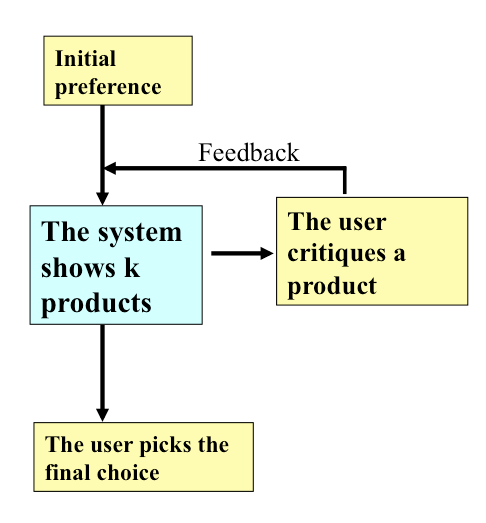
\includegraphics[width=1.0\textwidth]{critiquing.png}
\end{figure}

\begin{figure}
  \caption{Console Application - Offline Evaluation of the recommender system. Quality and Economy scores are initially set to 0.5, 0.5. The scores evolve in each iteration, depending on the product the user selects}
  \centering
    \includegraphics[width=0.8\textwidth]{evaluation.png}
\end{figure}


\end{document}



%Recommender systems are broadly classified into 3 categories:
%\begin{itemize}
%\renewcommand{\labelitemi}{$\bullet$}
%\item Collaborative recommmenders
%\item Content based recommenders
%\item Knowledge based recommenders
%\end{itemize}
%There are hybrid recommendation approaches proposed by combining techniques used in two or more of the recommender systems. Following is a brief description of  each of the categories:
%\subsubsection{Collaborative Recommender Systems:}
%Main idea of these systems here is that users who shared same interests in the past, will also share similar interests in the future.
%Advantages of collaborative systems are as follows:
%\begin{itemize}
%\renewcommand{\labelitemi}{$\bullet$}
%\item Data about systems need not be entered into the system and maintained
%\item Can capture many implicit factors involved in decision making, which are difficult to model in general
%\end{itemize}
%Challenges in the context of collaborative approaches include the following:
%\begin{itemize}
%\renewcommand{\labelitemi}{$\bullet$}
%\item How do we find users with similar tastes to the user for whom we need a recommendation?
%\item How do we measure similarity?
%\item What to do with new users who haven't given any ratings? How do we deal with items that no one has bought yet? (Cold start problem)
%\item What other techniques other than finding similar users can we use for making predictions?
%
%\end{itemize}
%
%\subsubsection{Content based recommender systems:}
%Content based recommendation is based on the availability of (manually created or automatically extracted) item descriptions and a model that captures the interests of a user.  Similar to item descriptions, user profiles may also be automatically derived and "learned" either by analyzing user behavior and feedback or by asking explicitly about interests and preferences. Advantages of content based systems are as follows:
%
%
%\begin{itemize}
%\renewcommand{\labelitemi}{$\bullet$}
%\item No cold start problem if a new item is added into the dataset
%\item It does not require large user group to achieve reasonable recommendation accuracy.
%\end{itemize}
%Following are the challenges faced in the context of content-based recommendation
%\begin{itemize}
%\renewcommand{\labelitemi}{$\bullet$}
%\item How do we automate acquisiton and continuously improve user profiles?
%\item How do we determine which items match, or are at least compatible with, a user's interests?
%\item What techniques can be deployed to automatically extract or learn the item descriptions to reduce manual annotation
%\end{itemize}
%
%\subsubsection{Knowledge based recommender systems:}
%In domains that involve a large number of one-time buyers like consumer electronics, cars etc, we cannot rely on existence of a purchase history, a prerequisite for collaborative and content-based filtering approaches.Typical customers buy a new camera only once every few years, so the recommender system cannot construct a user profile or propose cameras that others liked. In knowledge-based approaches, the recommender system typically makes use of additional, often manually provided, information about both the current user and the available items.
%Users also are willing to spend more time and express his preferences as precisely as possible. (Eg: The color of the car must be 'black' and price should be around \$5000 etc). This is the main reason why knowledge based recommender systems are characterized as \textit{conversational recommender systems}
%Following are the challenges faced in the context of knowledge-based recommendation
%\begin{itemize}
%\renewcommand{\labelitemi}{$\bullet$}
%\item Representation of knowledge in the knowledge base
%\item Which mechanism can be used to select and rank the items based on user's characteristics?
%\item How seriously can we take the customer's explicit preferences into account? Users typically have a poor domain knowledge and due to means-objectives(mistaking that one attribute positively correlates with another), he may express his preferences incorrectly
%\item What is the best interaction pattern that can be used for recommendation in a particular domain?
%\end{itemize}
